%!TEX root = ../systemnahe-programmierung.tex

\chapter{Projektidee}\label{projektidee}

\begin{figure}[htbp]
\centering
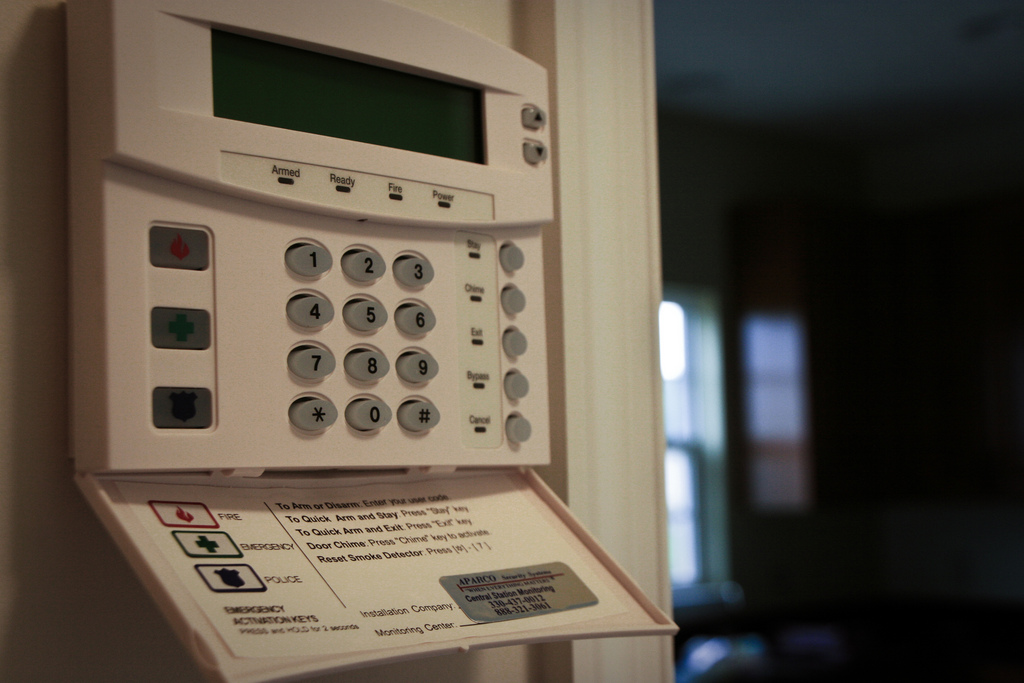
\includegraphics{images/keypad.jpg}
\caption[Nummerfeld einer Alarmsicherung]{Nummerfeld einer Alarmsicherung\footnotemark{}}
\end{figure}
\footnotetext{Quelle: https://www.flickr.com/photos/themillers91705/4916981638}

Bei einer Alarmsicherung meldet man sich normalerweise über ein Nummerfeld an, um den Alarmmodus an-
und auzuschalten. In diesem Projekt wollen wir eine einfaches Nummernfeld simulieren: Wenn man eine
vordefinierte 4-stellige Ziffernfolge eingiebt, kann man den Modus der Alarmsicherung ändern
(aus-/eingeschaltet).